\chapter{Einleitung}
\pagenumbering{arabic}
Die Studenten der Höheren Fachschule für Technik Mittelland (\acrshort{hftm}) aus der Studienrichtung Systemtechnik nehmen seit einigen Jahren am internationalen RoboCup teil. Dazu kommt ein Roboter mit selbst entwickelter Hard- und Software zum Einsatz. Unter dem Team-Namen ,,Solidus'' spielen die Studenten am RoboCup bereits an der Spitze mit (2. und 3. Platz). Das Team besteht nebst dem Dozenten Alain Rohr jedes Jahr aus neuen Studenten die keinen vertieften Hintergrund in der Softwareentwicklung haben. Sie übernehmen die bestehende Code-Base vom vorherigen Team und müssen diese an die neuen Gegebenheiten anpassen und erweitern. Beispielsweise ändert sich jährlich die Umgebung (Lichtverhältnisse, etc.), die Cup-Regeln und es müssen neue Sensoren oder Aktoren integriert werden. Die historisch gewachsene, monolithische Architektur der Software wirkt diesen Anforderungen aber entgegen.
Sie baten die BFH um Hilfe beim Software-Engineering. Es geht in dieser Arbeit also darum, ein Design für die Roboter-Software zu entwerfen, so dass die Studenten unabhängig voneinander entwickeln können.
\section{RoboCup}
Der RoboCup ist ein Wettbewerb, der seit 1997 jährlich ausgetragen wird \cite{wikipedia-robocup}. Ursprünglich ging es hauptsächlich darum, Roboter zu entwickeln, die gegeneinander Fussball spielen. Das langfristige Ziel dieses Wettbewerbs \cite{wikipedia-roboterfussball}: 
\begin{formal}
im Jahr 2050 den menschlichen Weltmeister in einem gewöhnlichen Fussballspiel zu schlagen
\end{formal}
Es kommen jedoch immer neue Ligen dazu. Der aktuelle Stand an Ligen für den RoboCup 2018 ist in Screenshot aus Abbildung \ref{fig:robocup_ligen} ersichtlich.
\begin{figure}[H]
	\centering
	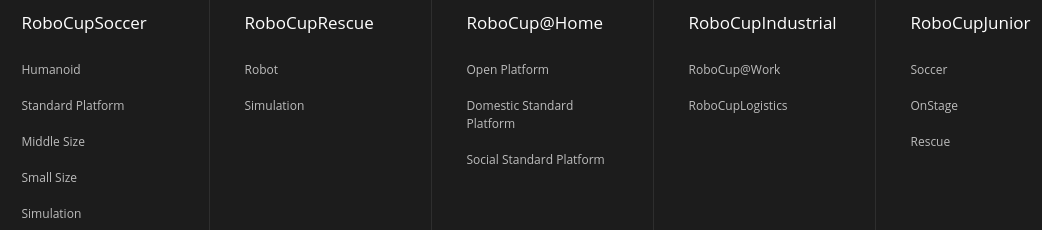
\includegraphics[width=\textwidth]{img/robocup-ligen.png}
	\caption{RoboCup Ligen, Screenshot von \cite{www.robocup.org}}
	\label{fig:robocup_ligen}
\end{figure} 
So gibt es beispielsweise in der Disziplin ,,RoboCupSoccer'' die Liga ,,Humanoid''. Die Roboter aus dieser Liga sind auch in den Medien hierzulande sehr bekannt. Im Bild \ref{fig:robocup_fussball} ist ein solcher Humanoid beim Fussballspielen am RoboCup zu sehen.
\begin{figure}[H]
	\centering
	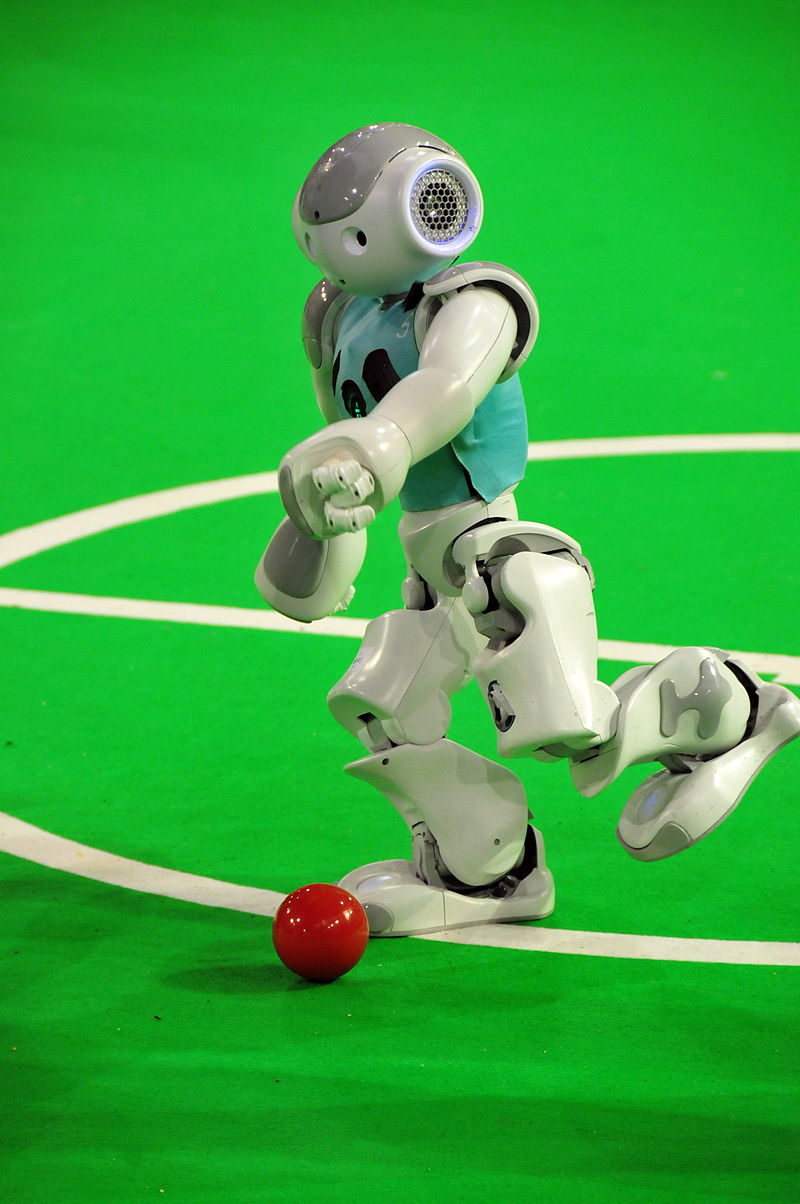
\includegraphics[width=0.2\textwidth]{img/robocup-humanoid.jpg}
	\caption{Roboter beim Fussball spielen. Quelle: Ralf Roletschek / roletschek.at \cite{robocup2013}}
	\label{fig:robocup_fussball}
\end{figure}
\subsection{RoboCupLogistics}
Seit 2012 gibt es am RoboCup die Liga ,,Logistics'', die wie folgt spezifiziert ist \cite{wikipedia-robocup}:
\begin{formal}
	Ziel dieser Liga ist die Entwicklung von autonom agierender Roboter zur Steuerung des Material- und Informationsflusses in industriellen Produktionsanlagen.
\end{formal}
Es spielen zwei Teams gegeneinander mit jeweils 3 Robotern. Auf dem  Spielfeld (Abbildung \ref{fig:robocup_spielfeld} und \ref{fig:robocup_spielfeld-real}) sind pro Team zufällig sieben Maschinen  aufgestellt. Diese müssen von den Robotern erkundet werden. Dafür hat jede Maschine vorne und hinten einen eindeutigen 2D-Code aufgedruckt, dem so genannten AR Tag (Prinzip ähnlich einem QR-Code). Jede Maschine repräsentiert eine Station in einer Produktionsanlage (einer ,,smart factory''). An jeder Station können Gegenstände zugebracht und auf der gegenüberliegenden Seite entnommen werden. Kontrolliert, überwacht und bewertet wird das Spiel von der ,,Referee Box''. Von ihr werden die 'Active orders' (Bestellungen) verwaltet und publiziert, die die Roboter auf dem Spielfeld umsetzen müssen. Sie koordiniert auch die Maschinen auf dem Spielfeld, zu denen die Roboter fahren müssen, um Gegenstände zu bringen und abzuholen.
\begin{figure}[H]
	\centering
	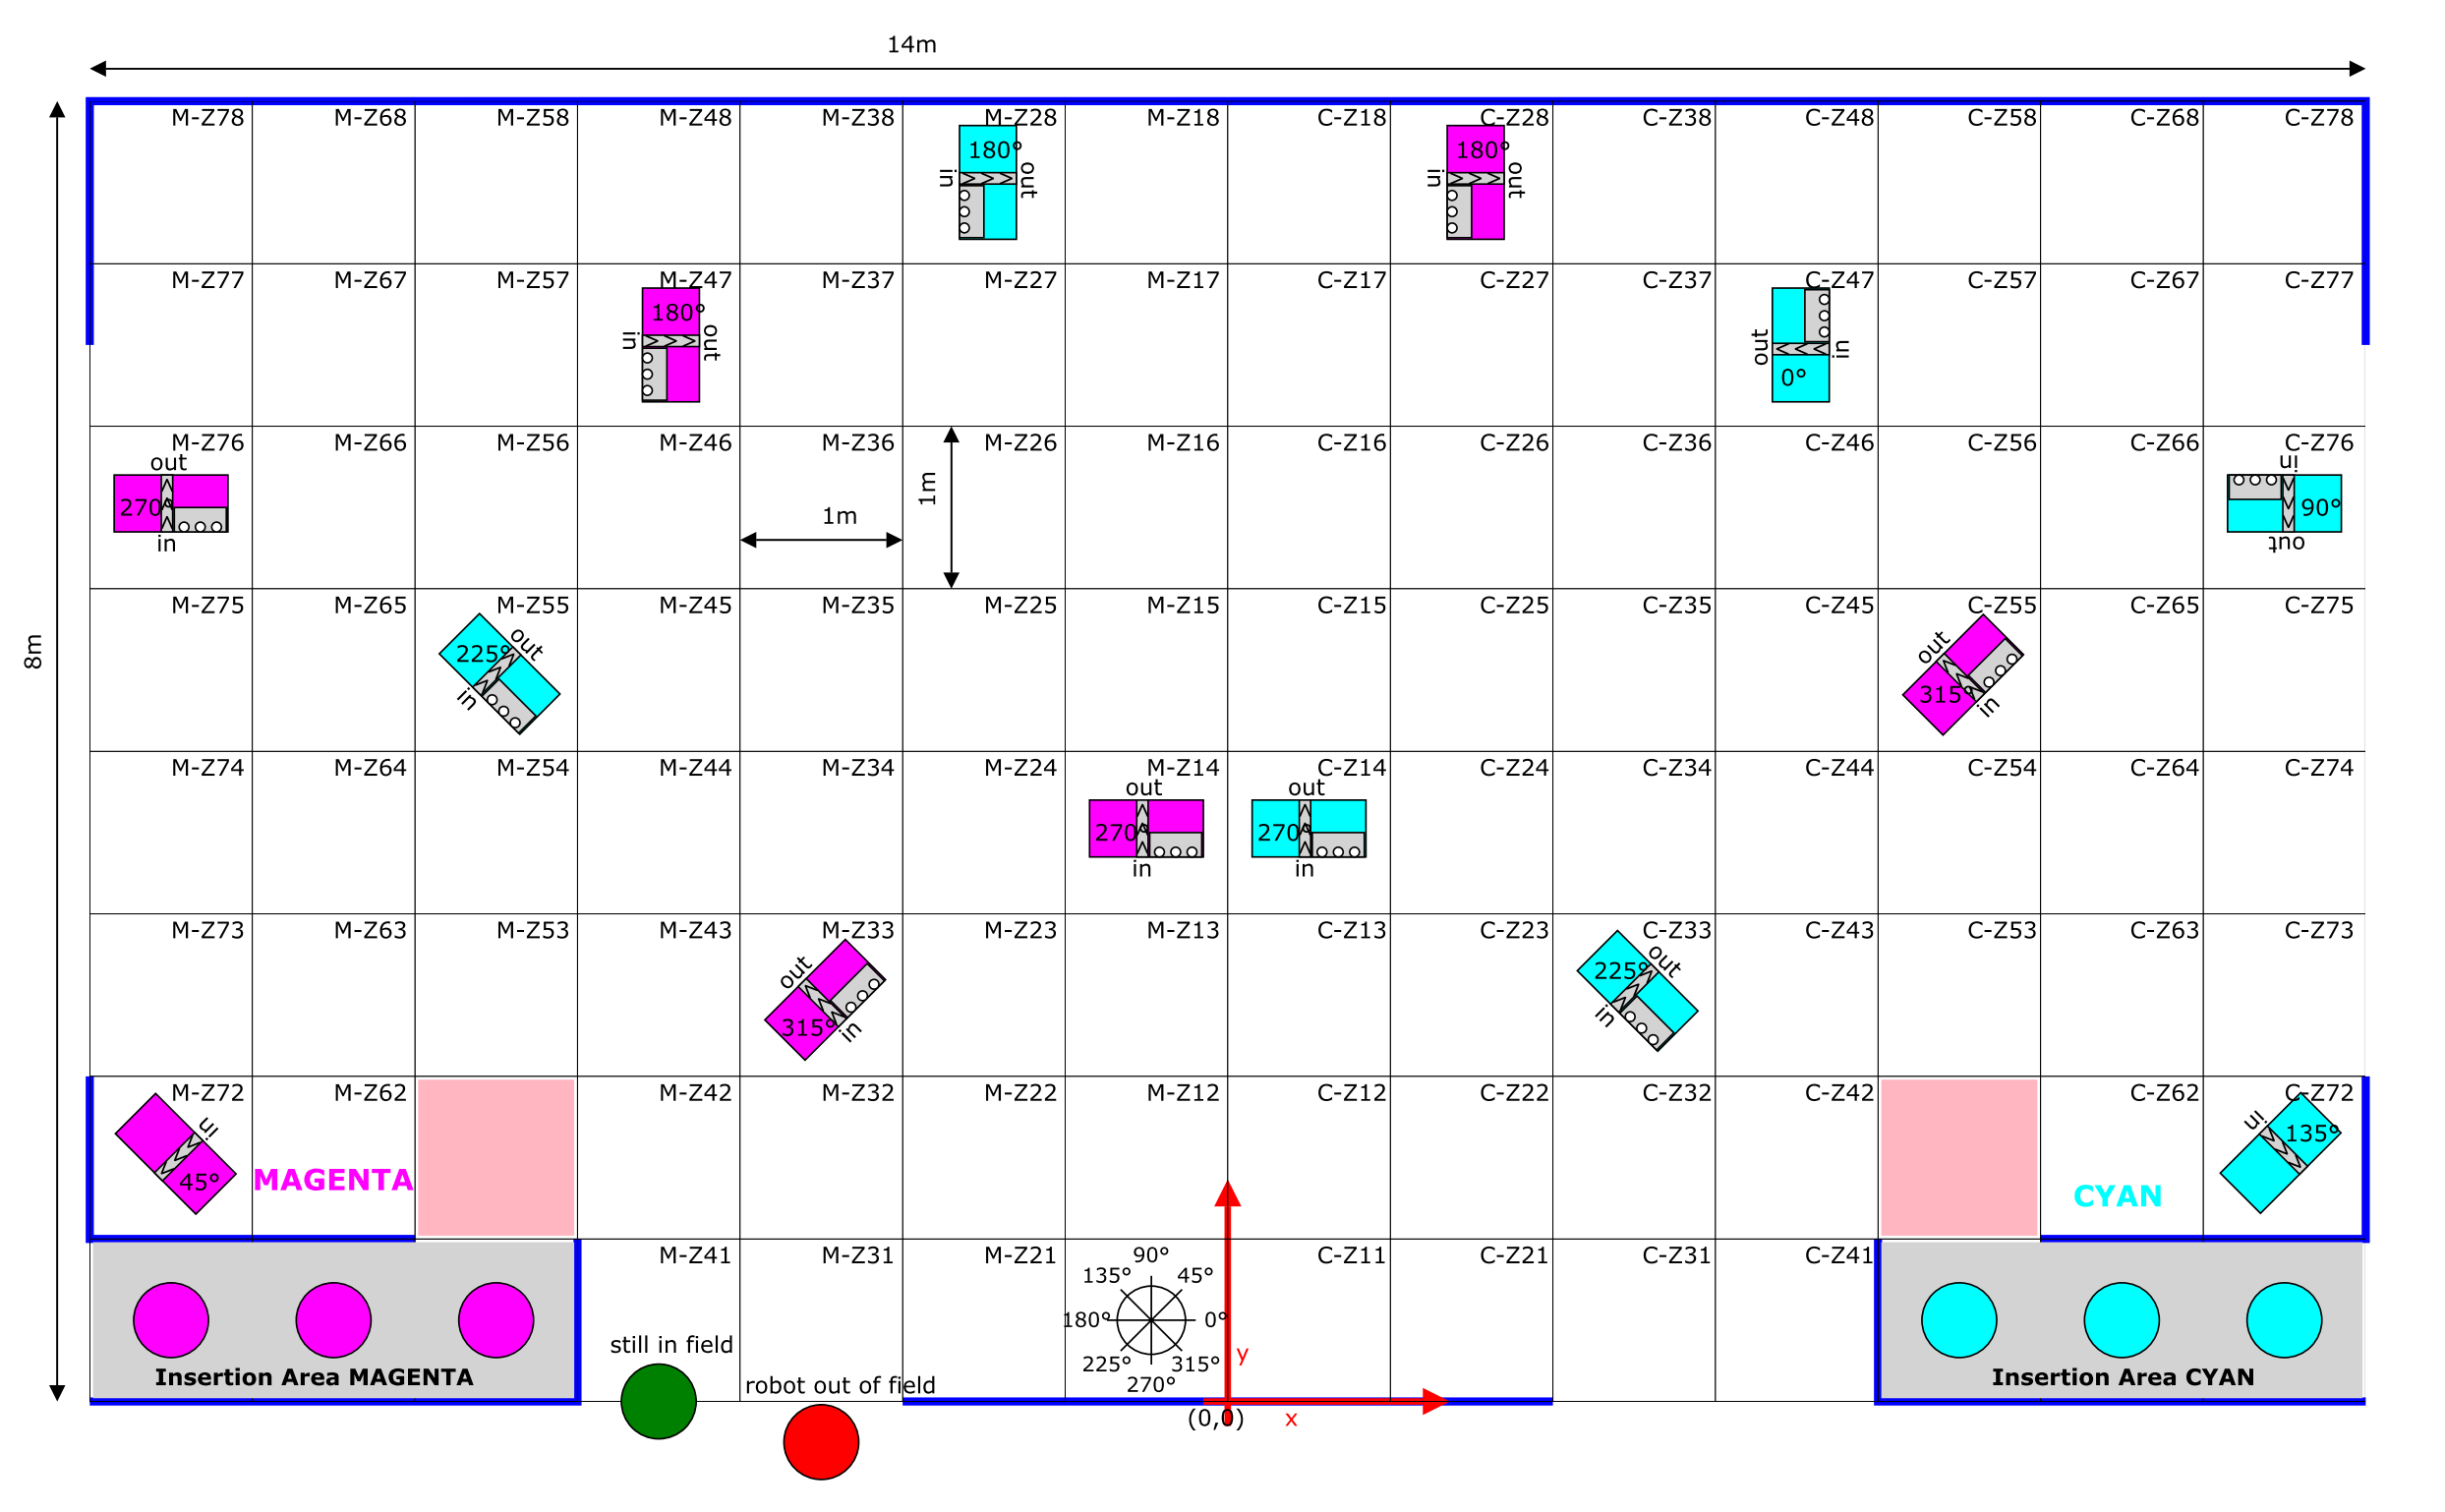
\includegraphics[width=0.75\textwidth]{img/robocup-spielfeld-2d.png}
	\caption{Spielfeld mit möglicher Aufstellung der Maschinen: Quelle: robotics-erlangen.de \cite{robotics-erlangen.de}}
	\label{fig:robocup_spielfeld}
\end{figure}

\begin{figure}[H]
	\centering
	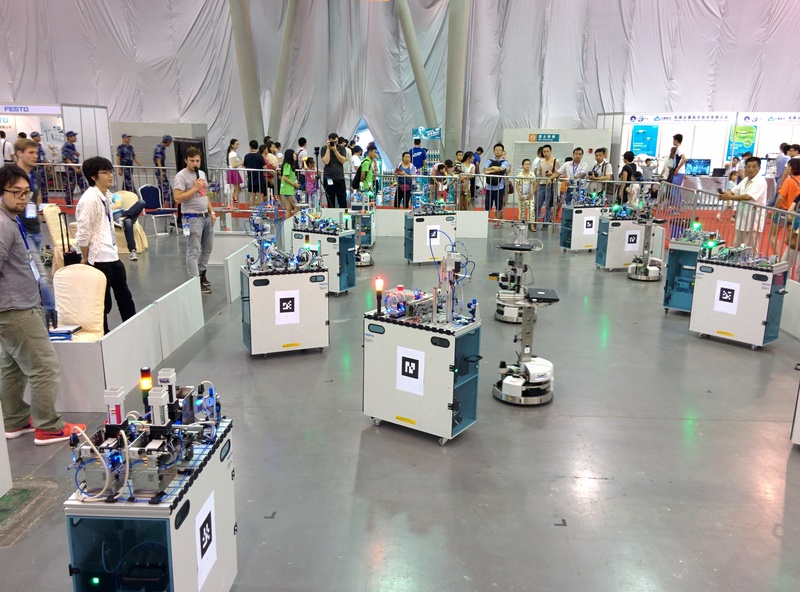
\includegraphics[width=0.75\textwidth]{img/robocup-in-action.jpg}
	\caption{Blick aufs Spielfeld während dem Wettbewerb Quelle: carologistics.org \cite{carologistics-blog}}
	\label{fig:robocup_spielfeld-real}
\end{figure}

Die verwendeten Roboter in dieser Liga basieren auf der ,,Robotino''-Plattform  von Festo (Abbildung \ref{fig:robotino}), die den Wettbewerb auch mit den Maschinen und anderem sponsern. Auf dieser Roboterplattform können verschiedene Sensoren, Aktoren und Computer-Systeme angebaut werden.
\begin{figure}[H]
	\centering
	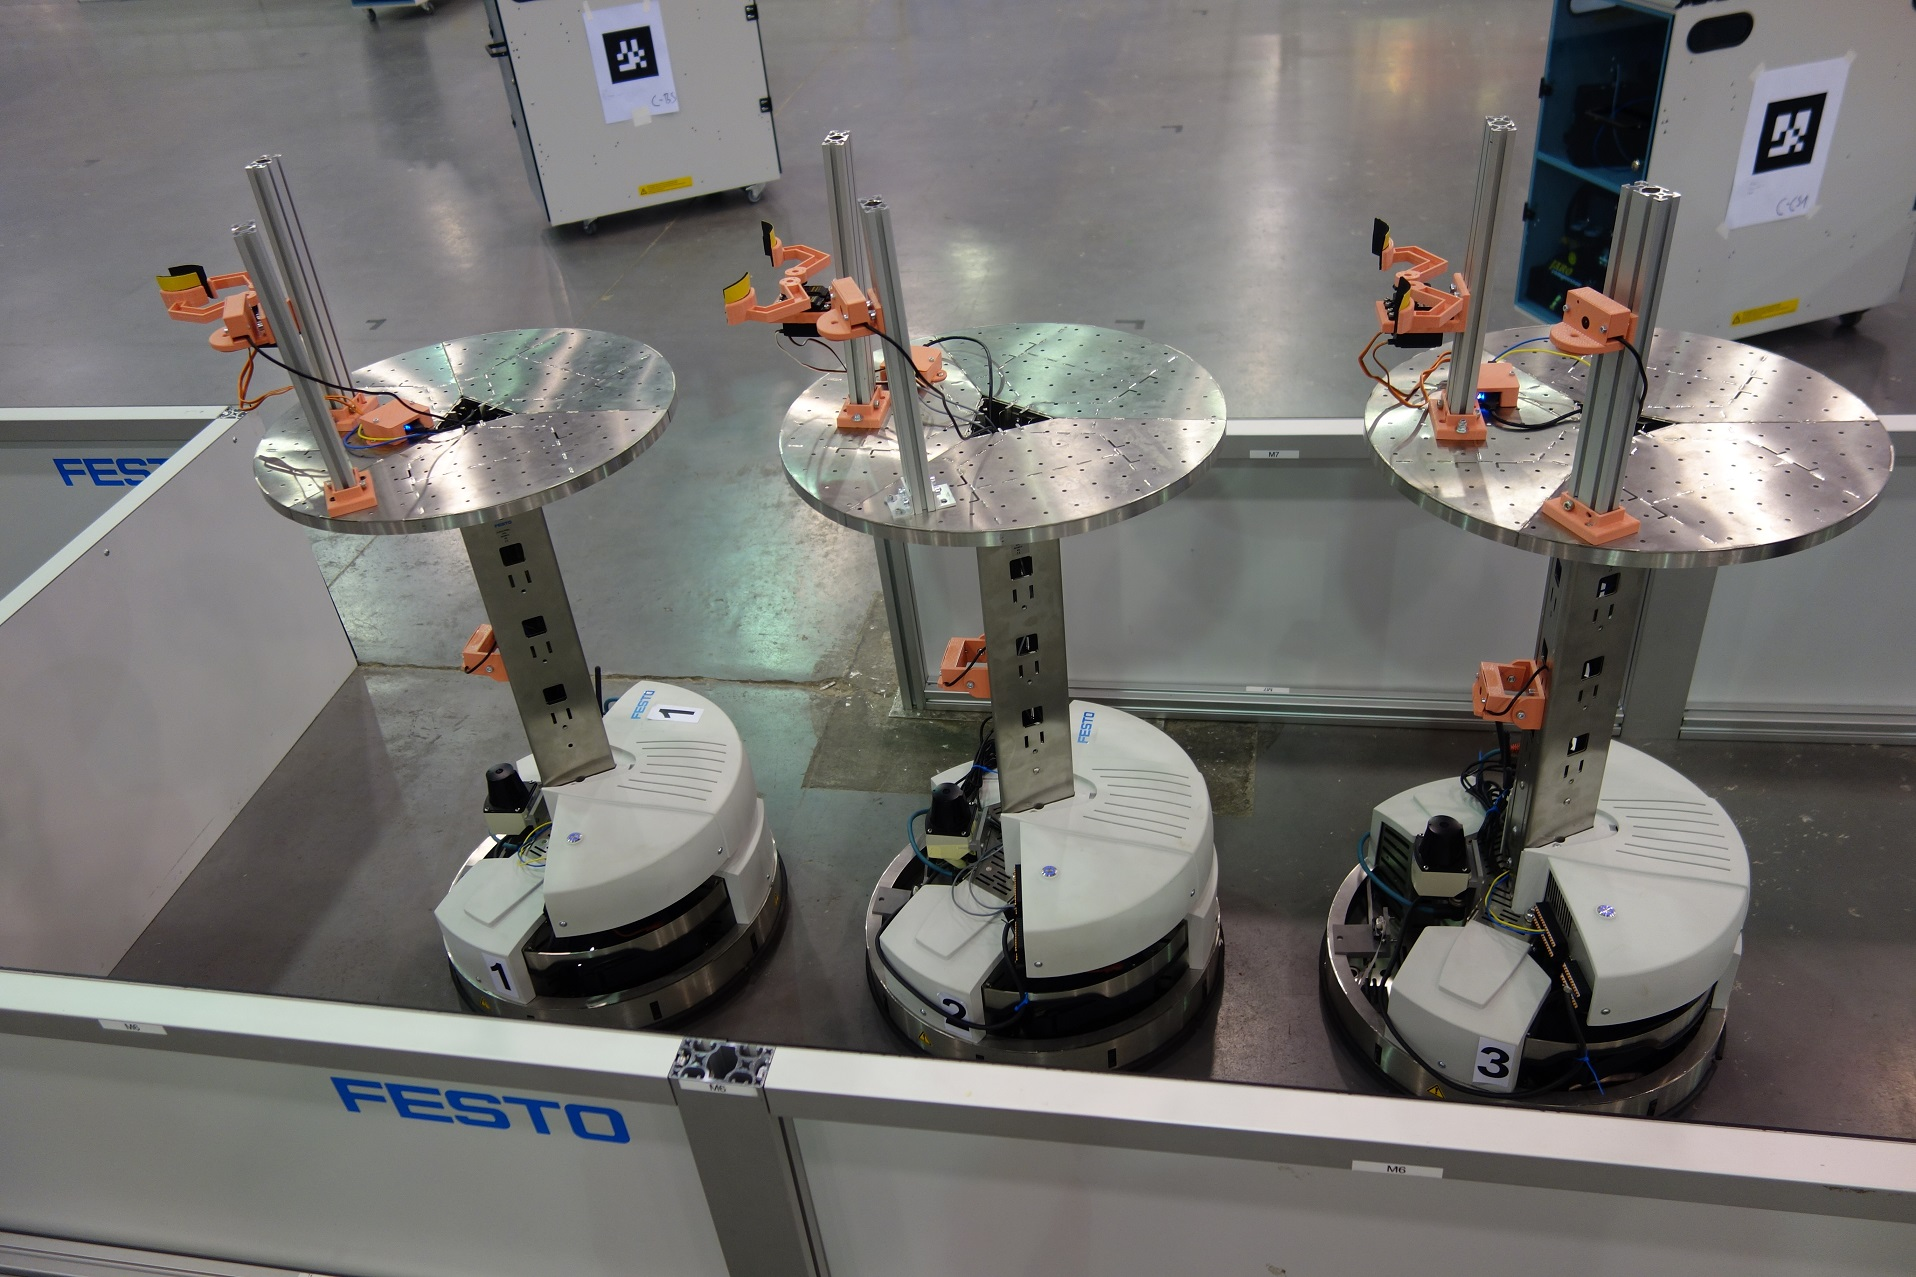
\includegraphics[width=0.5\textwidth]{img/robotino_v3.jpg}
	\caption{Robotino v3 für die Logistics League\cite{robotino}}
	\label{fig:robotino}
\end{figure}



\section{\acrshort{lidar}}
Diese Arbeit zeigt anhand eines \acrshort{lidar}-Sensors, wie ein mögliches Software-Design für den Roboter aussehen kann. Doch was ist \acrshort{lidar}?
\begin{formal}
	Lidar ist eine dem Radar verwandte Methode zur optischen Abstands- und Geschwindigkeitsmessung sowie zur Fernmessung atmosphärischer Parameter. Statt der Radiowellen wie beim Radar werden Laserstrahlen verwendet. \cite{wikipedia-lidar}
\end{formal}
Meistens versteht man unter em Begriff \acrshort{lidar} gleich einen Sensor, wie er auch in dieser Arbeit verwendet wird. Sie messen nicht nur in eine Richtung, sondern fast die ganze Umgebung um den Sensor herum. Der in dieser Arbeit verwendete TiM55x kann 270° der Umgebung ausmessen. Solche Sensoren kommen beispielsweise bei Fahrzeugen mit Autopilot (Bsp. Tesla) zum Einsatz um die Hindernisse in der Umgebung zu erkennen. Im Prinzip funktionieren solche Sensoren ähnlich wie eine Radar-Bodenstation in der Luftfahrt: Über ein drehendes Element (bei \acrshort{lidar} einen Spiegel) werden kontinuierlich Laserstrahl-Impulse ausgesendet. Wenn sich ein Objekt in der Nähe des Sensors befindet, trifft dieser Laserstrahl das Objekt und ein Teil davon wird reflektiert. Die Reflexion detektiert der Sensor und errechnet daraus die resultierende Distanz zum Objekt.
\begin{figure}[H]
	\centering
	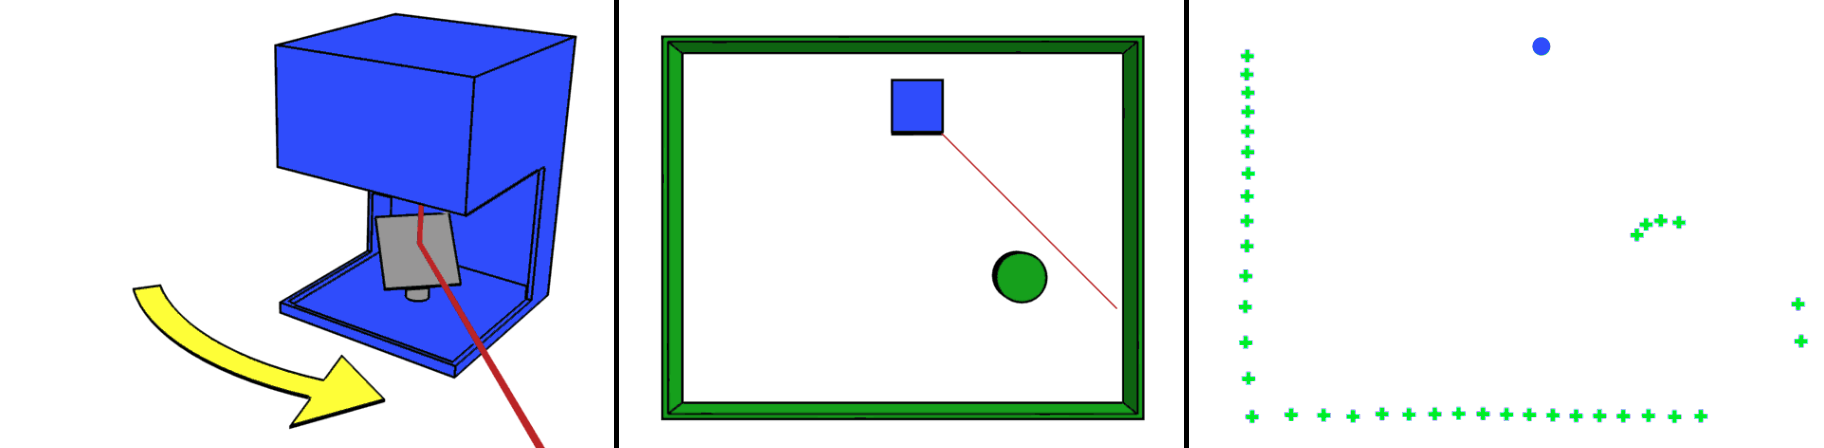
\includegraphics[width=0.7\textwidth]{img/lidar-principle.png}
	\caption{Prinzip 2D-Abtastung mit Lidar \cite{wikipedia-lidar}}
	\label{fig:lidar-principle}
\end{figure}


\subsection{SICK TiM55x}
\label{chap:tim55x}
Die Funktionsweise des verwendeten Sensors ist im Datenblatt vom Hersteller SICK wie folgt beschrieben \cite{tim55x-techinfo}:
\begin{formal}
Der TiM5xx sendet mit einer Laserdiode gepulste Laserstrahlen aus. Trifft ein solcher Laserpuls auf ein Objekt oder eine Person, wird er an dessen Oberfläche reflektiert. Die Reflexion wird im Empfänger des TiM5xx von einer Fotodiode registriert. Der TiM5xx nutzt die SICK-eigene HDDM-Technologie (High Definition Distance Measurement). Bei diesem Messverfahren wird ein Messwert durch die Mittelwertbildung mehrerer Einzelpulse gebildet. Aus der Laufzeit, die das Licht von der Aussendung des Strahls bis zum Empfang der Reflexion benötigt, berechnet der TiM5xx die Entfernung zum Objekt. Dieses Prinzip der ,,Pulslaufzeitmessung'' wird in ähnlicher Form von Radarsystemen benutzt.

Mit einem rotierenden Spiegel lenkt der TiM5xx die ausgesendeten Laserstrahlen ab und tastet damit die Umgebung radial ab. Die Messungen werden intern von einem Winkelkodierer in regelmässigen Winkelschritten ausgelöst. Eine komplette Rotation stellt einen Messvorgang (Scan) dar. Der TiM5xx arbeitet mit einer Scanfrequenz von 15 Hz, d. h. er durchläuft 15 Messvorgänge pro Sekunde und stellt die Messergebnisse fortlaufend in Echtzeit über die Ethernet-Schnittstelle zur Verfügung.
\end{formal}

Wir erhalten also von diesem Sensor 15 Mal pro Sekunde eine komplette Messung mit 270 Distanzen und der dazugehörigen Genauigkeit. Diese Messwerte sind wie im Datenblatt beschrieben wie folgt zu verstehen: Den ersten Messwert erhalten wir bei -45° und den letzten bei 225° (siehe dazu Abbildung \ref{fig:lidar}). Der TiM55x-Sensor ist an der Robotino-Plattform so verbaut, dass 90° vorne entspricht. Weshalb der Hersteller negative Werte im Koordinatensystem verwendet hinterfragen wir nicht weiter. Die zu entwickelnde Software soll also genau diesen Winkel-Bereich zur Verfügung stellen - so steht er auch im Datenblatt.
\begin{figure}[H]
	\centering
	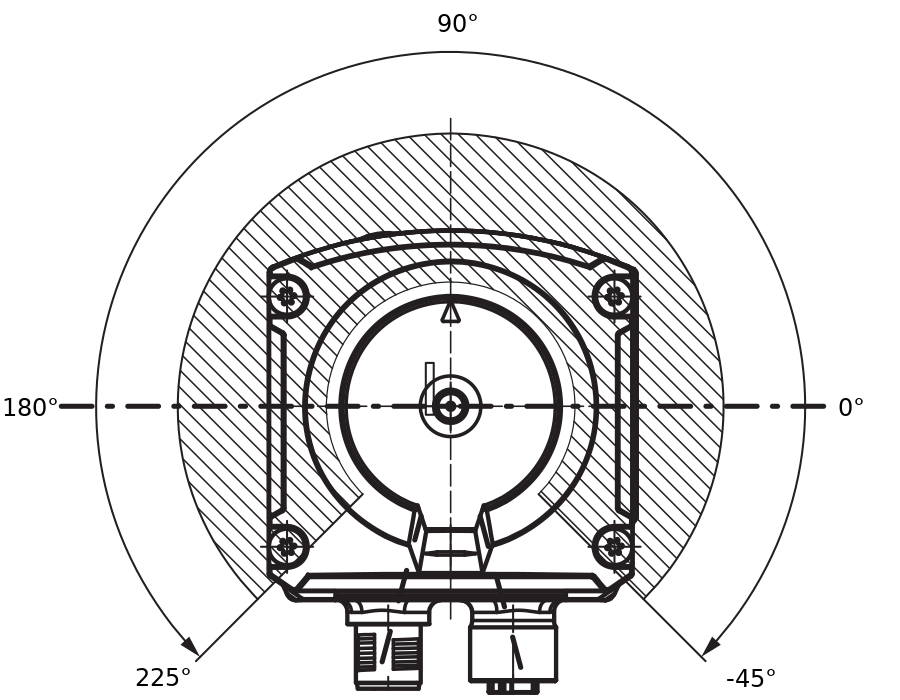
\includegraphics[width=0.5\textwidth]{img/lidar-coordinate.png}
	\caption{\acrshort{lidar}: Draufsicht / Koordinatensystem}
	\label{fig:lidar}
\end{figure}
